\section{Bionische Oberflächen 2}

\subsection{Temporäre Haftsysteme mit regulierbaren Hafteigenschaften}

\textit{Beispiel 1: Klettverschluss.} Nach dem Vorbild von Klettfrüchten, deren Samen durch das Klettsystem (kleine Widerhaken) an Tieren anhaften und sich verbreiten. Als biologisches Vorbild dienen die Hakenstrukturen von Spreizklimmern.
\\
\textit{Verbesserungen vom Klettverschluss}:
\begin{itemize}
    \item Mit richtungssabhängigen, variablen \& richtungsabhängigen Hafteigenschaften: Pneumatische Schläuche öffnen die Haken unter Druck ($\rightarrow$ Haftung).
    \item \textbf{Anisotrope (richtungsunabhängige) Haftung} \dangersign: Je nach Bewegungsrichtung Haften oder Gleiten. Beste Eigenschaften, wenn weiche Fasern in steife Fasern greifen $\rightarrow$ zB für Posterclips.
\end{itemize}

\begin{center}
    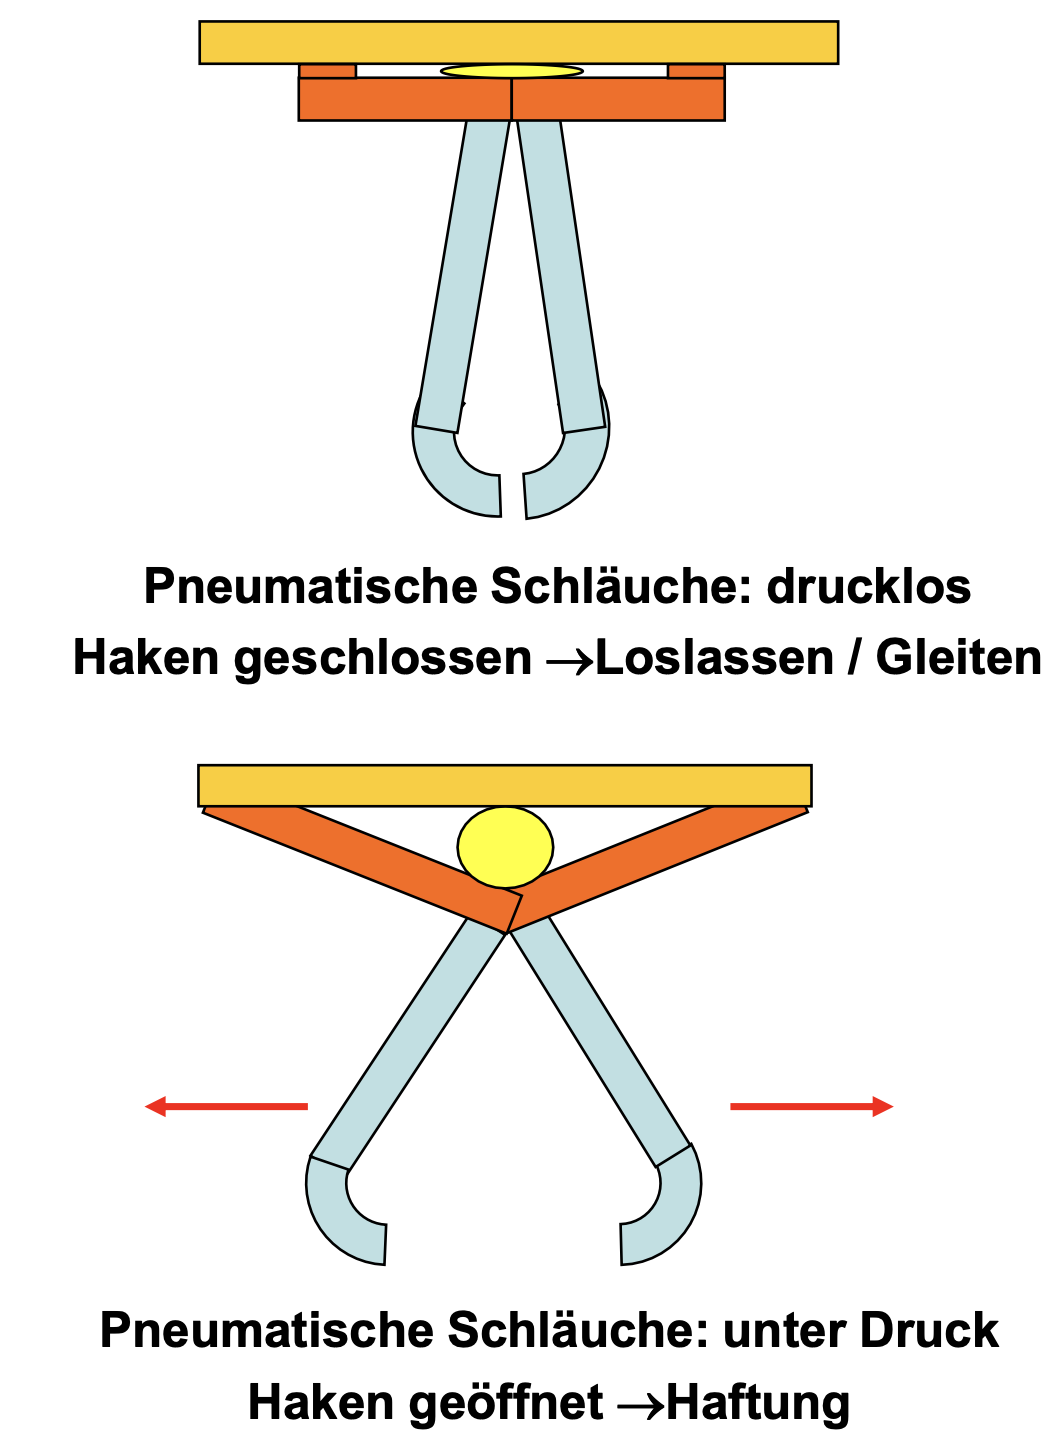
\includegraphics[width=4cm]{lec4/figures/pneumatik.png}
    \hfill
    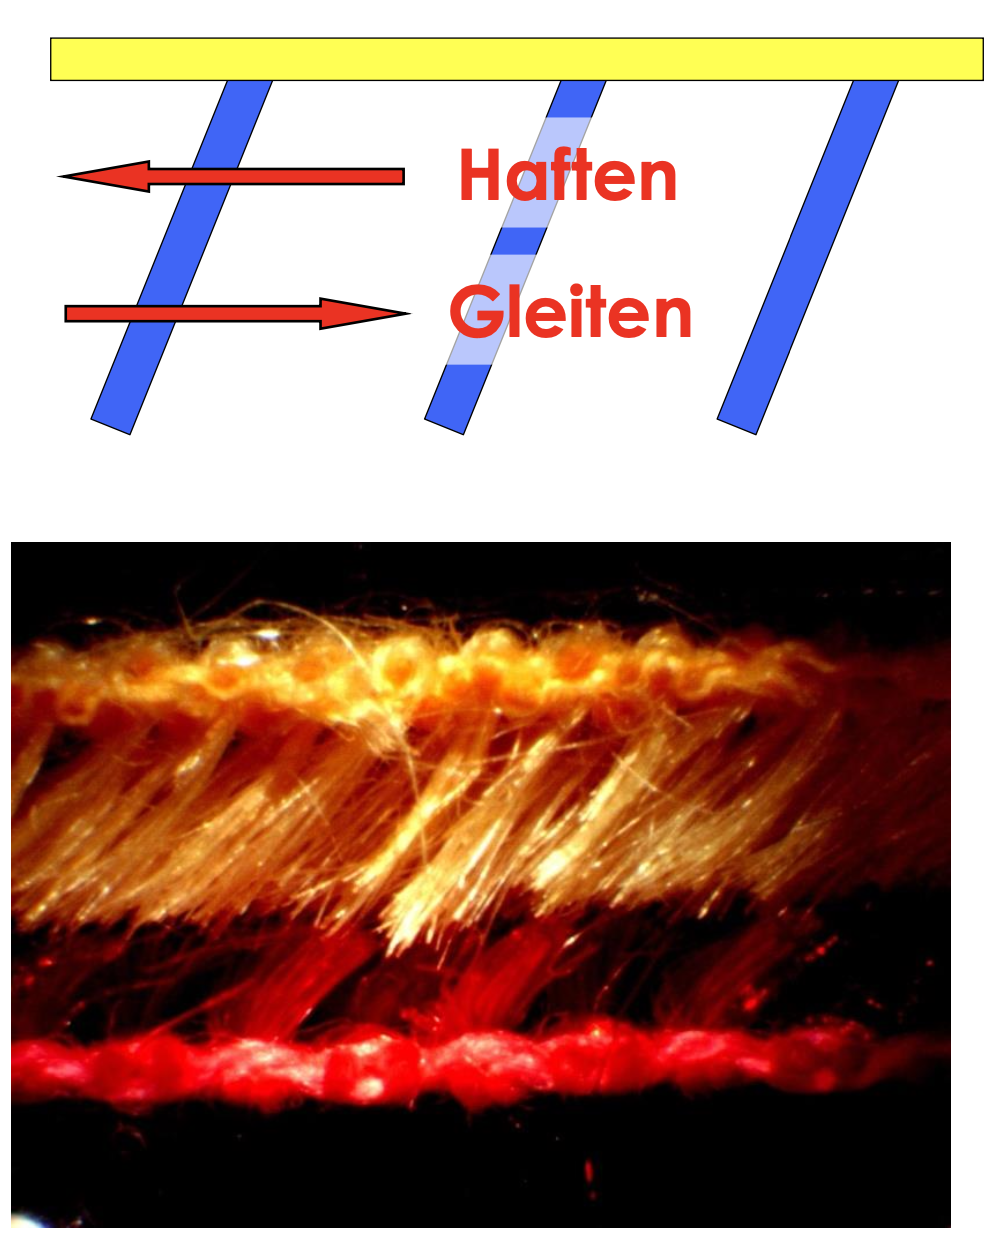
\includegraphics[width=4cm]{lec4/figures/anisotropes_haften.png}
\end{center}

\subsection{Permanente Haftsysteme mit hoher Haftkraft}

\textbf{Beispiel 1: Haftwurzeln beim Efeu.} Das Wurzelhaar wächst in Spalten ein, nimmt mit dem Substrat Kontakt auf und klappt durch Eintrocknen um $\rightarrow$ Haftung. In den Haaren sind die Fasern in 30-40° zur Längsrichtung orientiert, aber in der Sitze in 60° $\rightarrow$ verursacht das Abknicken in der Spitze. Zudem hat der Efeu ``Klebekapseln'' die die Wurzelhaare an das Substrat binden. Bei Kraft-Weg-Messungen an Hauswänden zeigt sich ein abgestuftes Versagen. An Baumborken werden höhere Haftkräfte erreicht, wobei durch das weichere Substrat schnelleres Versagen eintritt.
\\
(\dangersign\textit{Wie haftet Efeu? Warum knickt es ab? Wo haftet es besonders gut? $\rightarrow$ raue Oberflächen hoher Festigkeit})

\begin{center}
    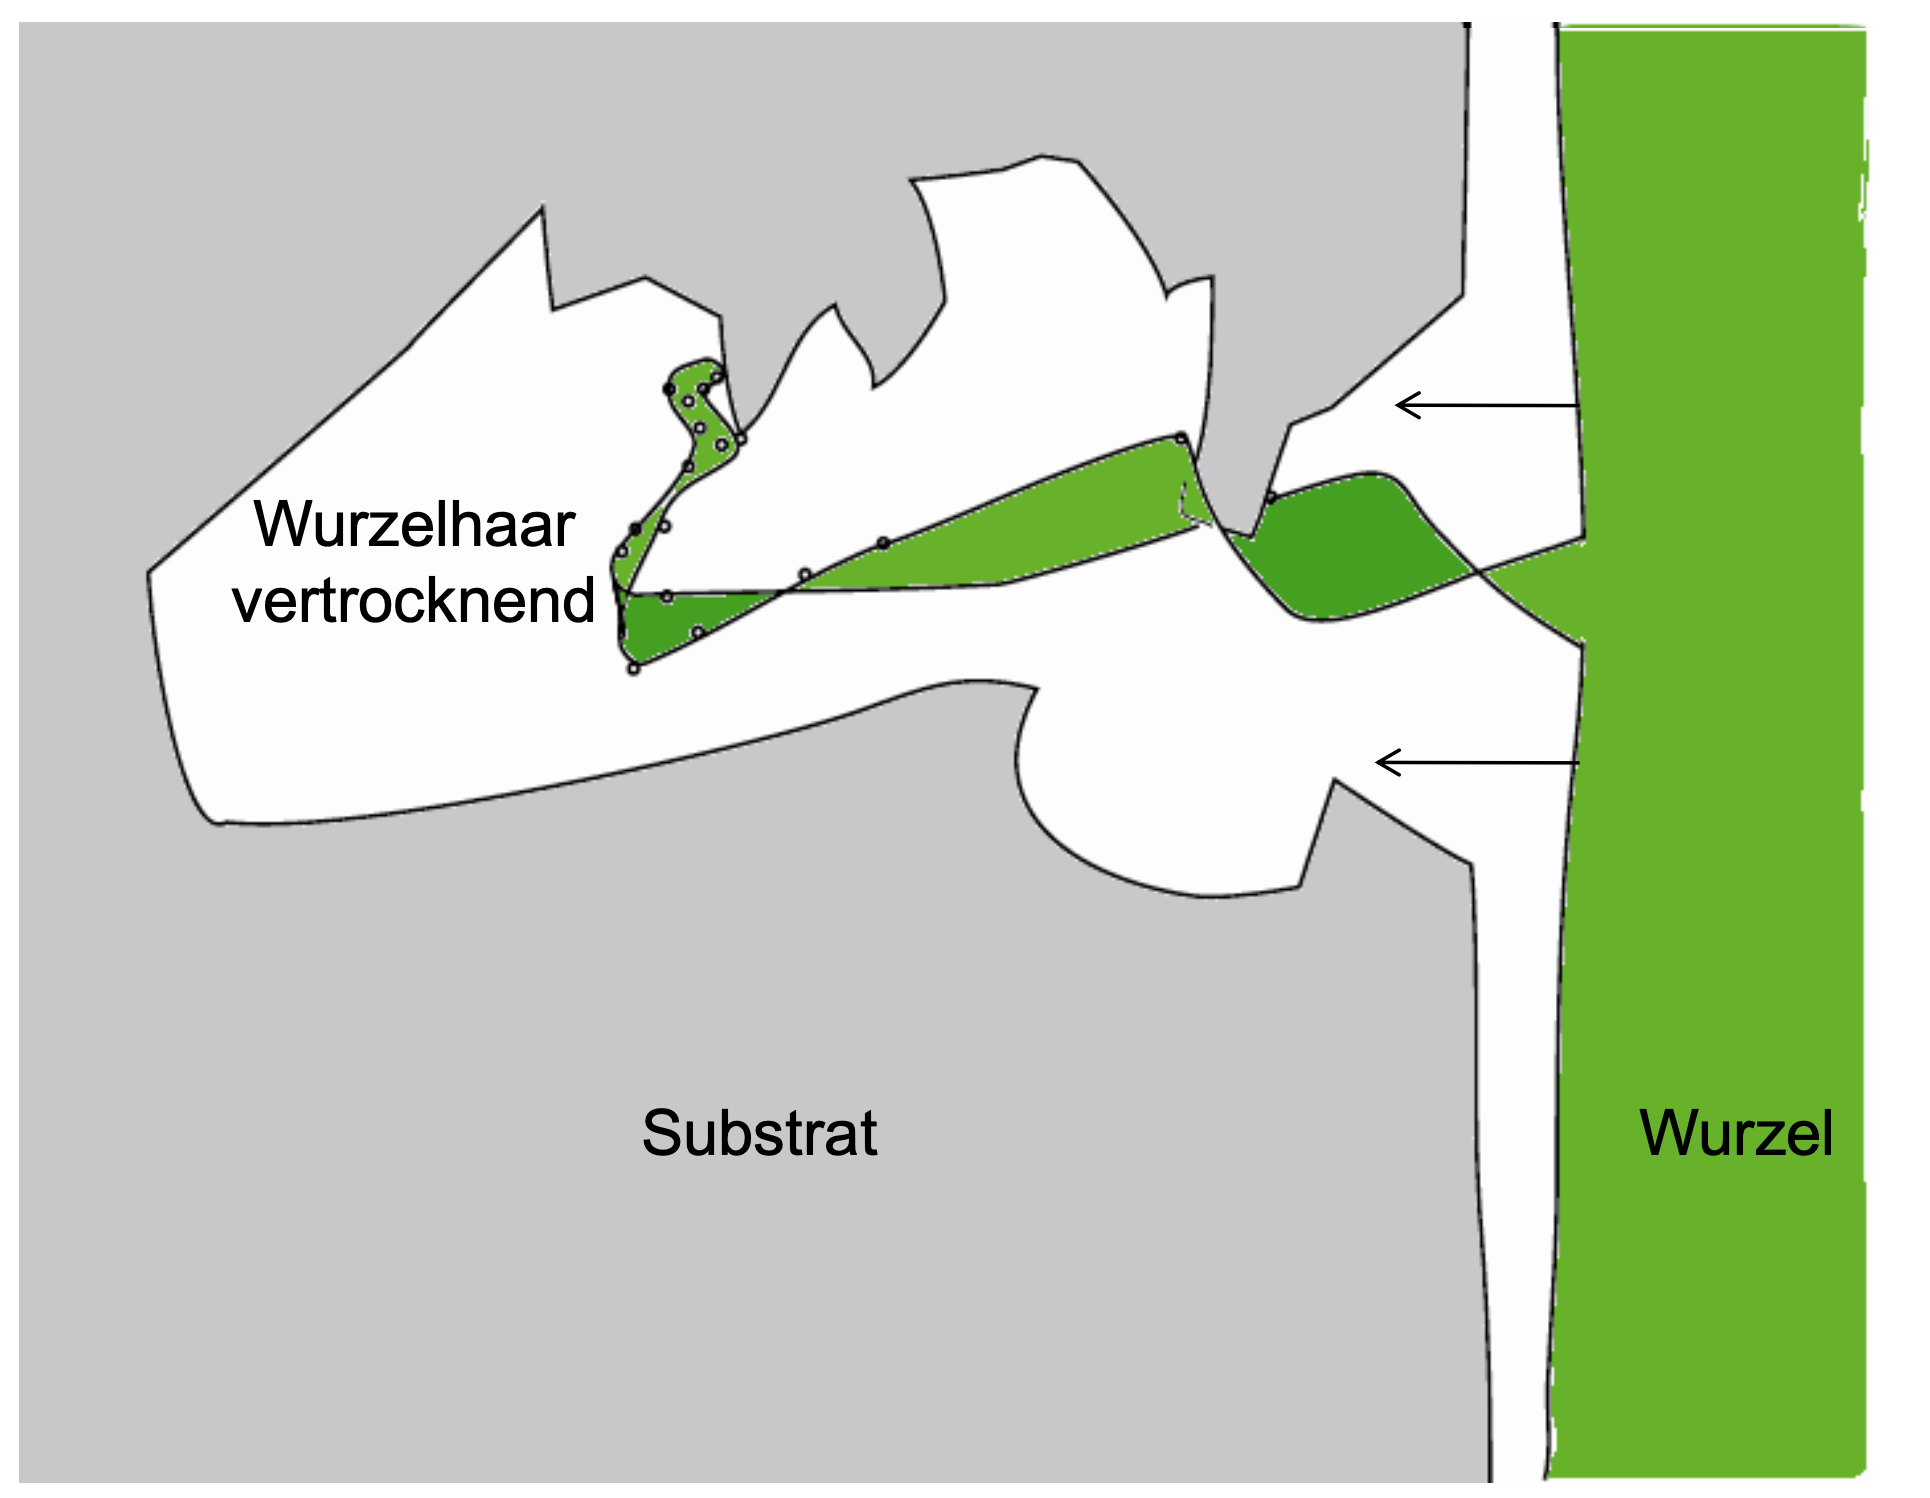
\includegraphics[width=5cm]{lec4/figures/efeu_haar.png}
    \hfill
    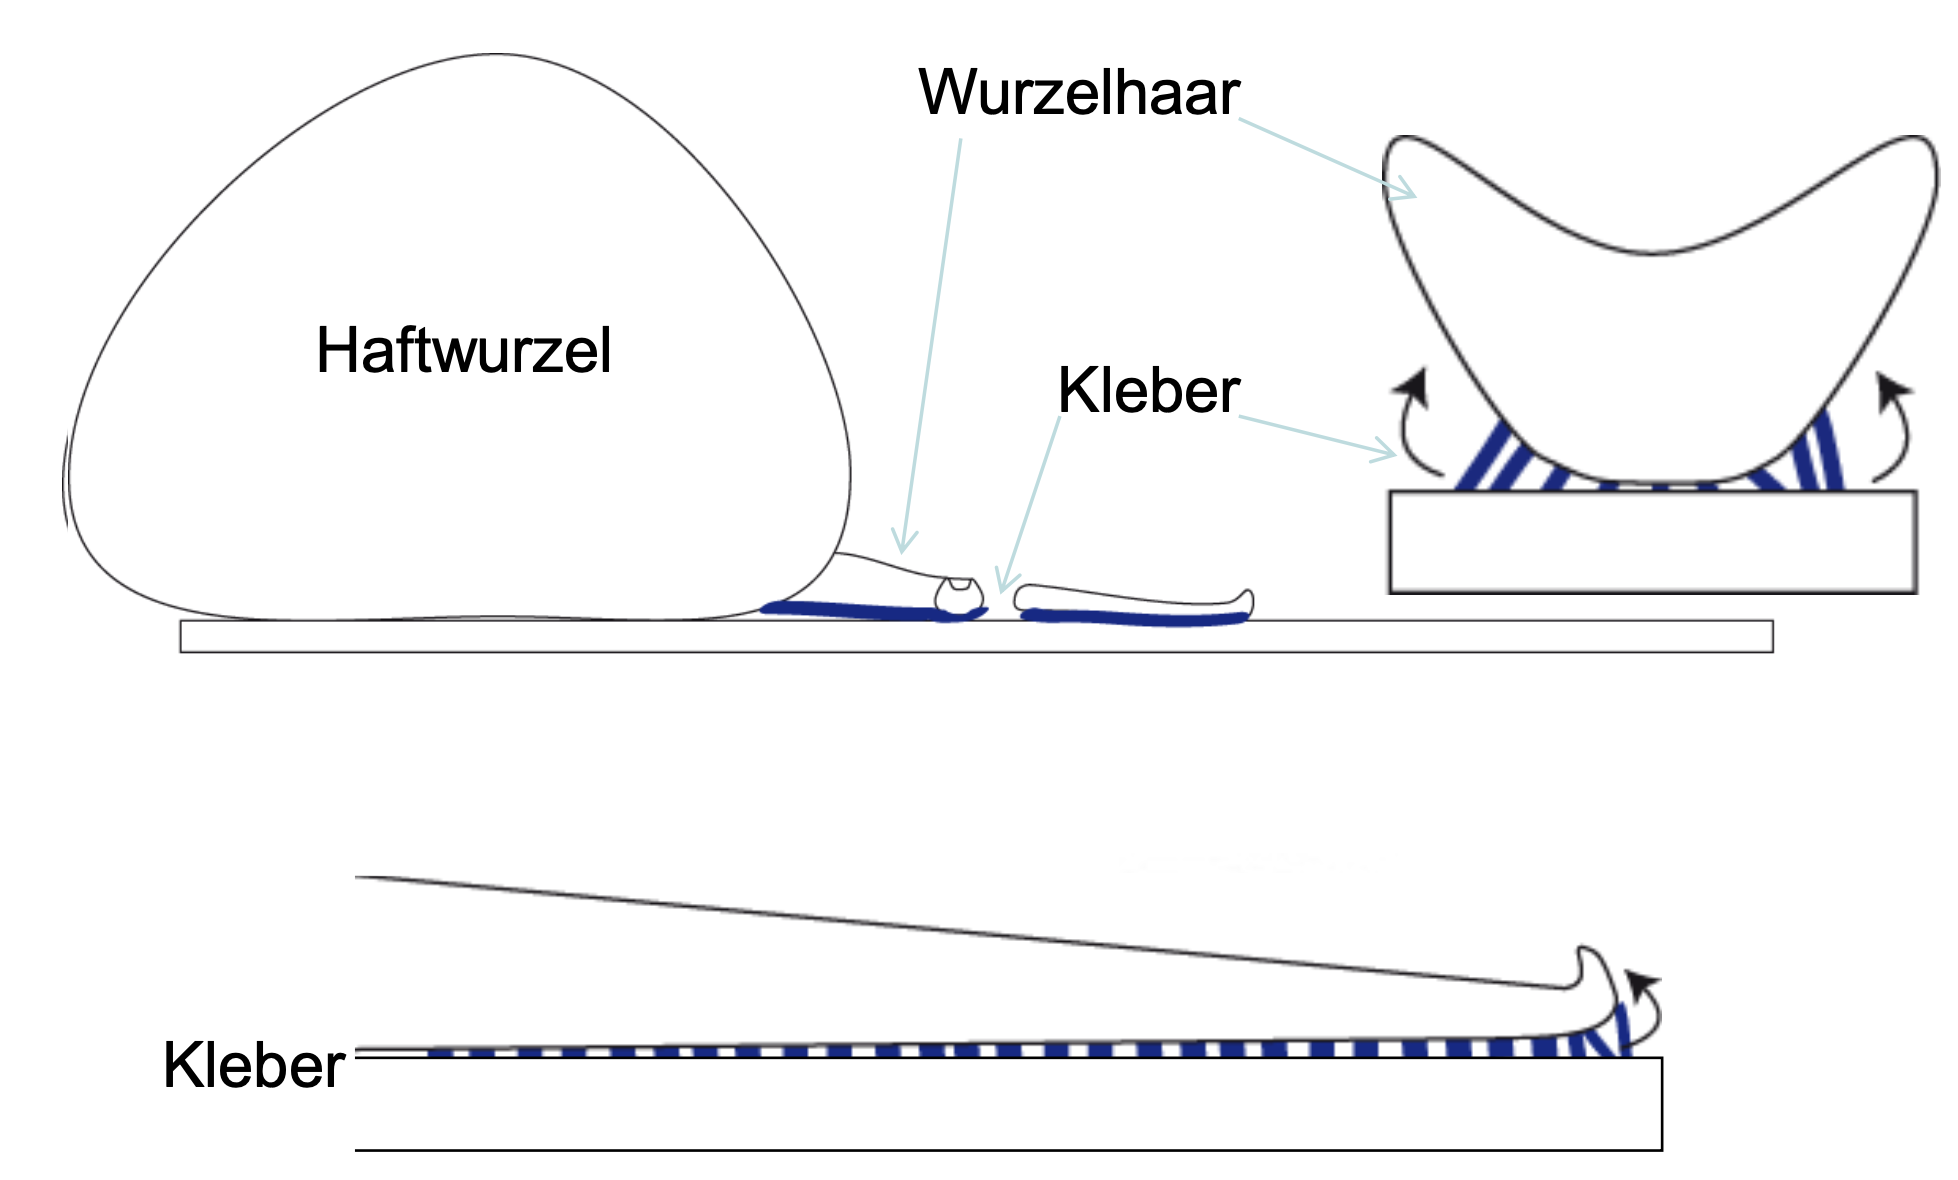
\includegraphics[width=5cm]{lec4/figures/efeu_kleber.png}
    \hfill
    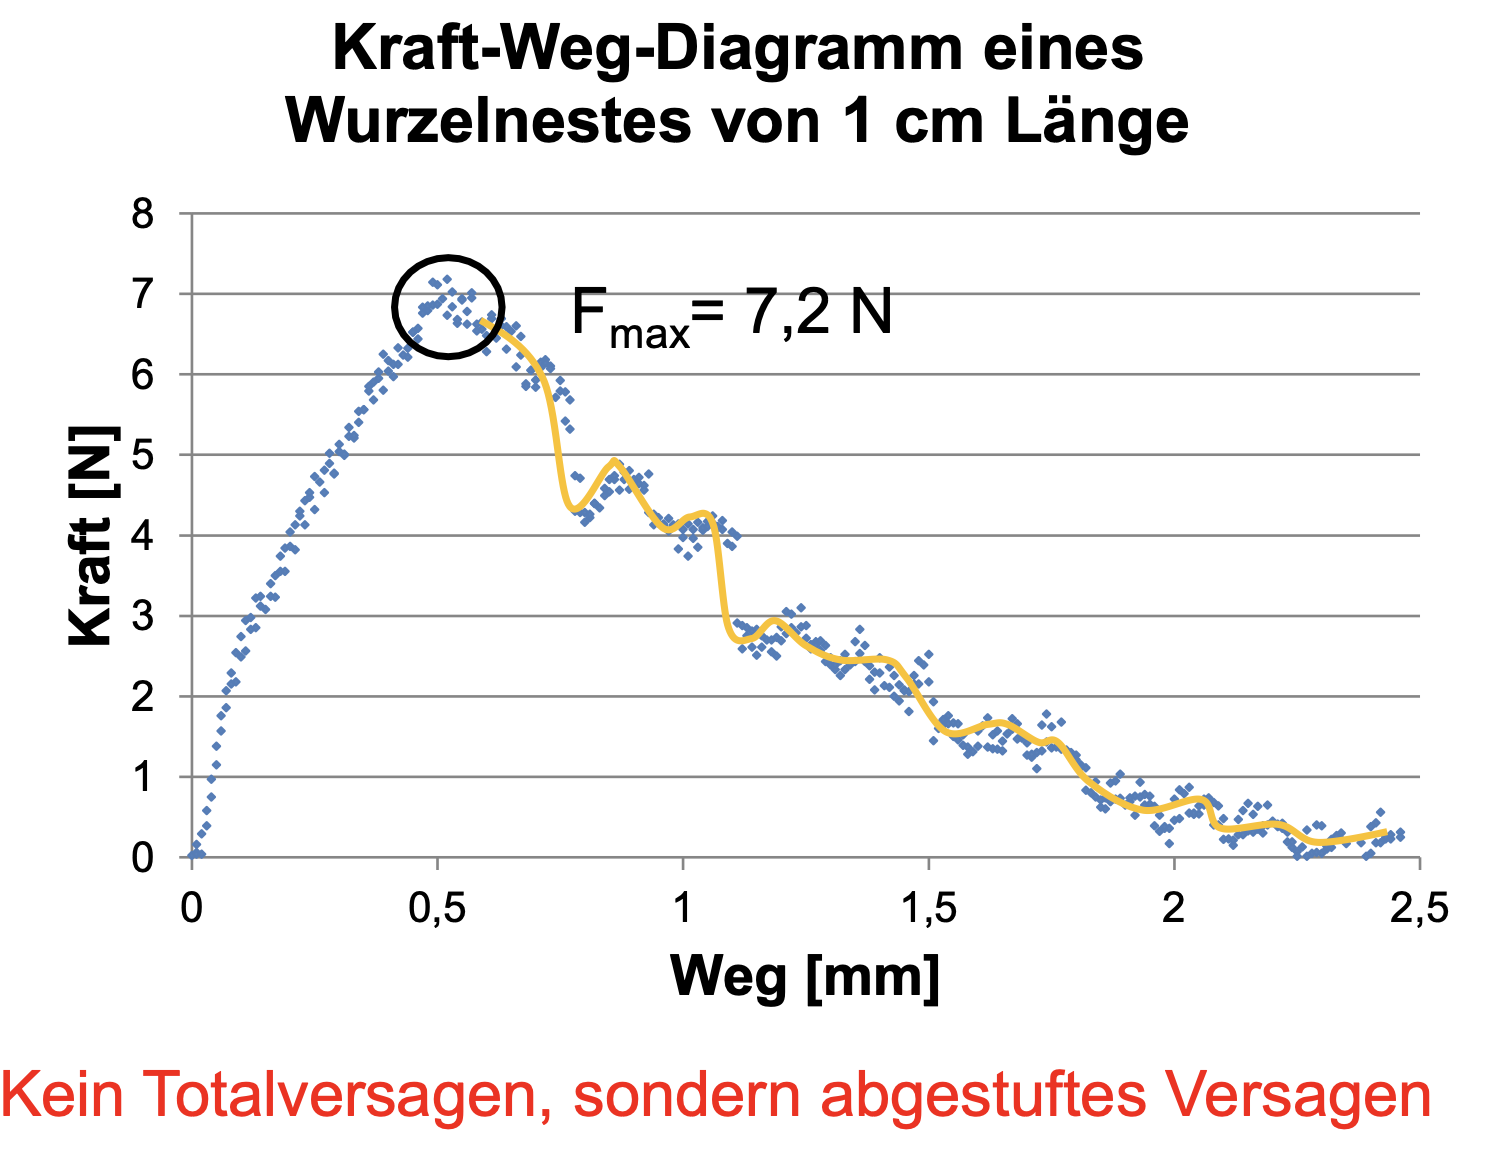
\includegraphics[width=5cm]{lec4/figures/efeu_versagen.png}
\end{center}
\textbf{Beispiel 2: Haftpads beim Wilden Wein.} Ranken wachsen $\rightarrow$ kommen in Kontakt zum Substrat $\rightarrow$ Haftpads bilden Hüte aus $\rightarrow$ Haftpads verholzen. Im Gegensatz zum Efeu zeigt das Kraft-Weg-Diagramm beim Wilden Wein Totalversagen. Je nach Art des Substrats stellen sich dabei unterschiedliche Versagensbilder ein (auf Putz versagt eher das Substrat und auf Aluminium versagt eher die Kappe).

\textit{Bionische Umsetzung:} Es wird probiert, Kleber in die Kontaktzone zweier Oberflächen so einzubringen, sodass die Kraftleitungsgeometrie der Haftpads beim Wilden Wein imitiert wird.

\begin{center}
    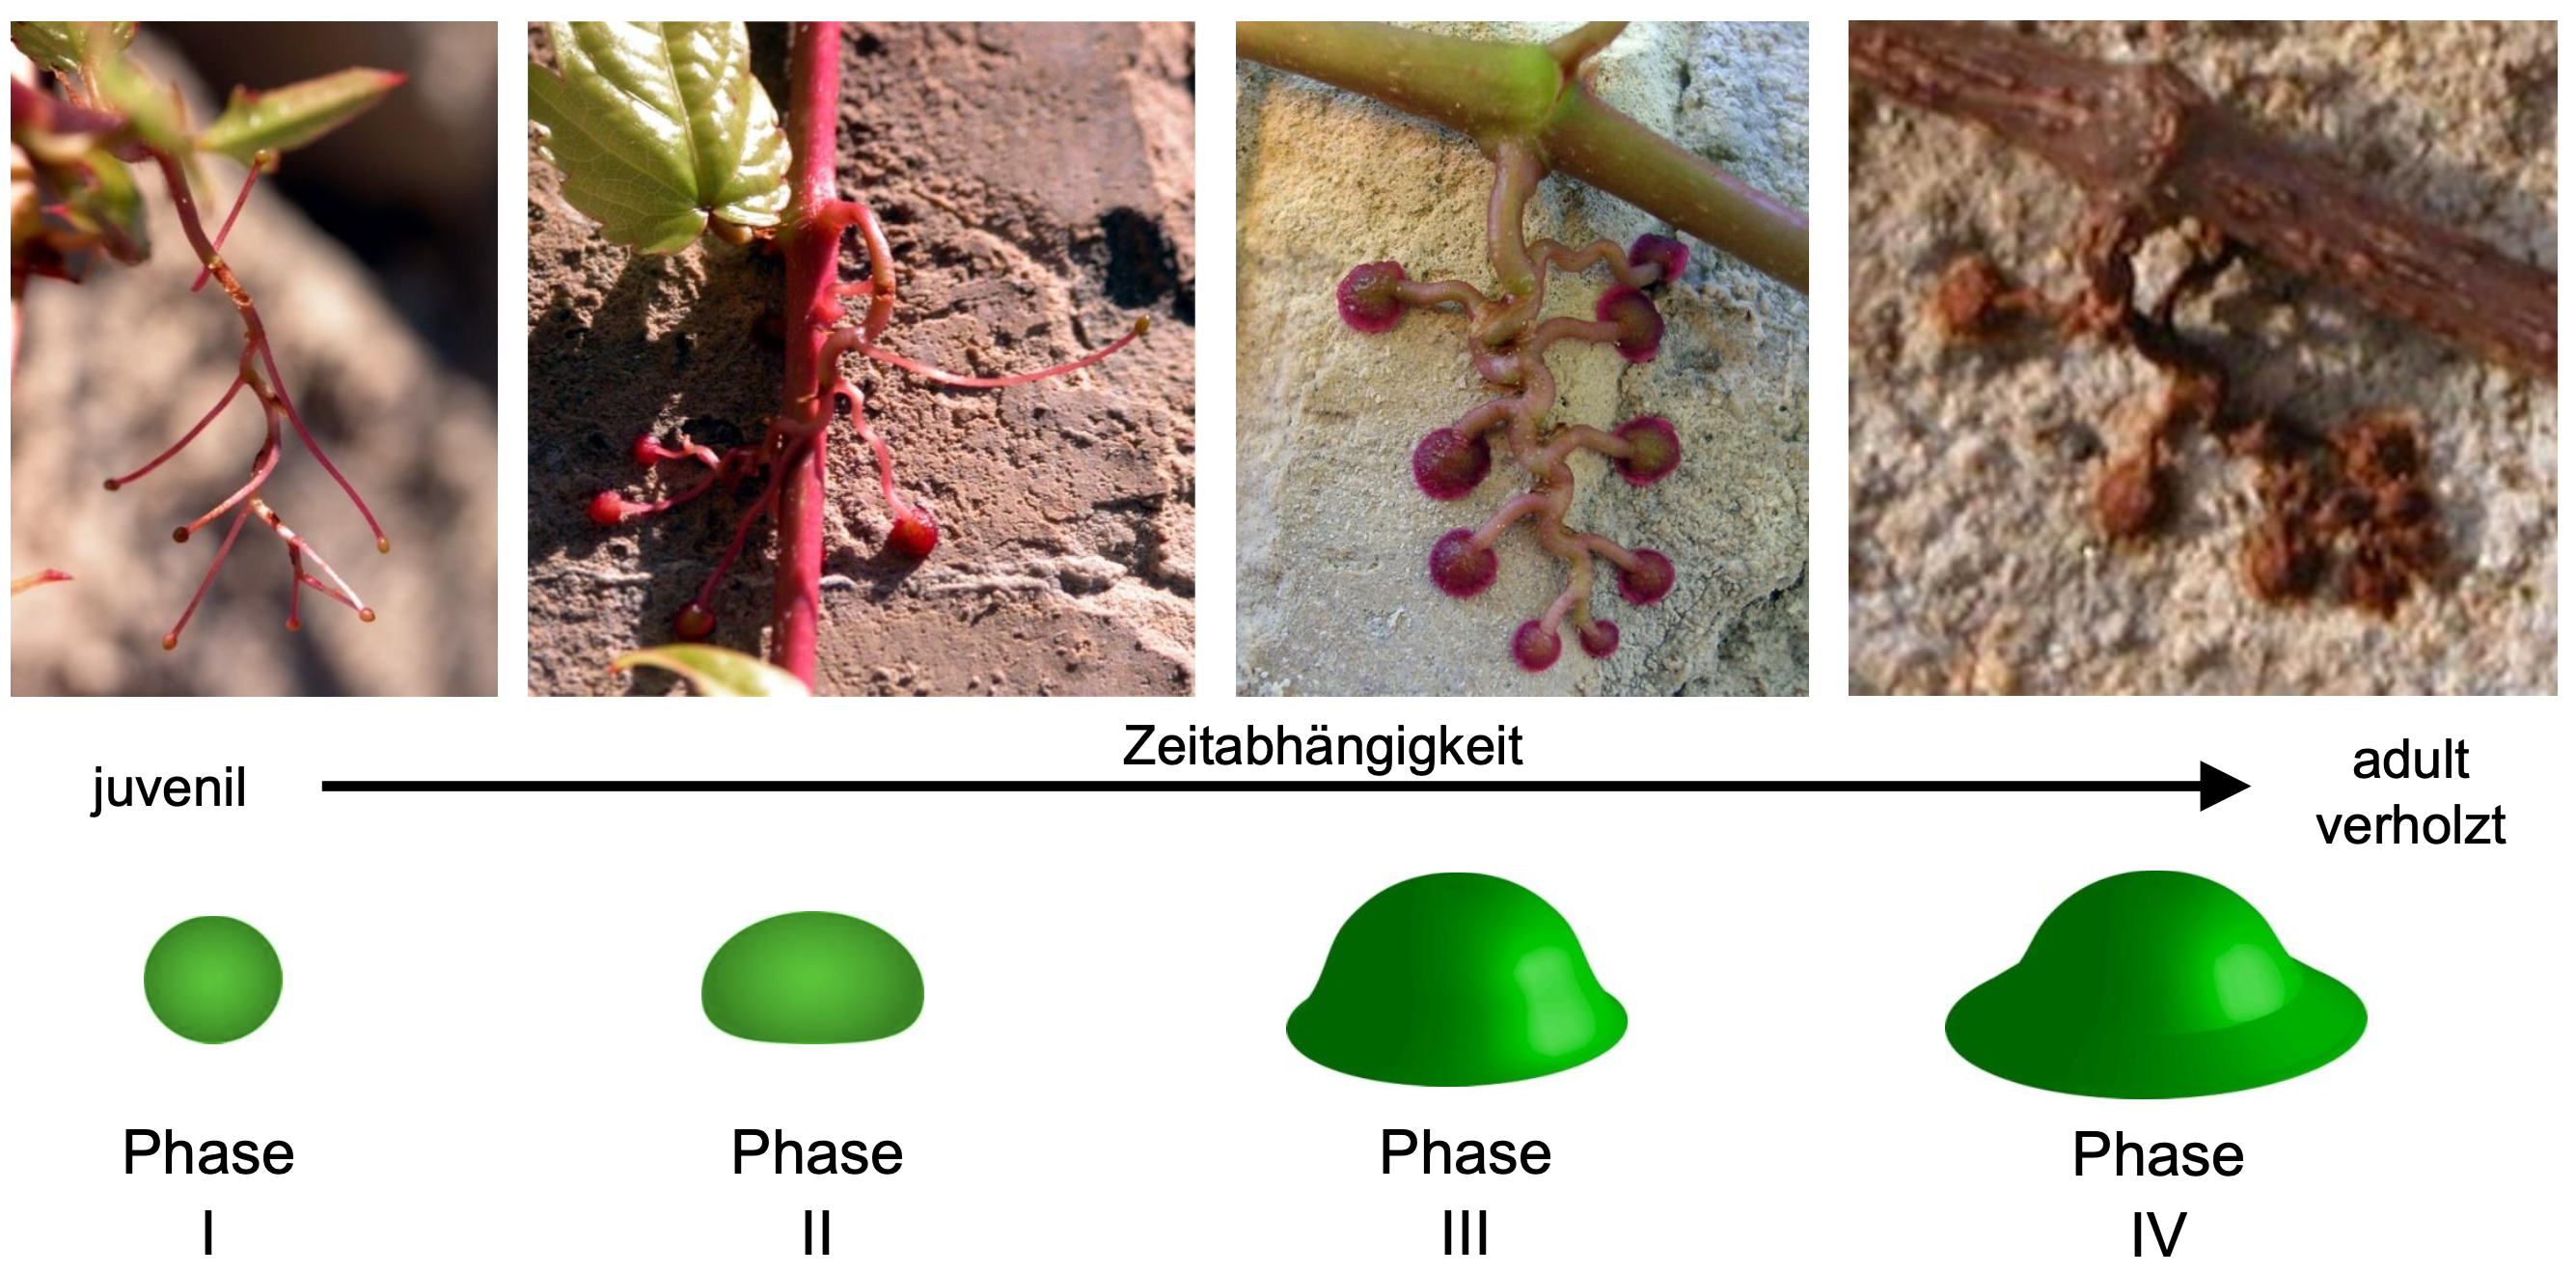
\includegraphics[width=9cm]{lec4/figures/wein_zeit.png}
    \hfill
    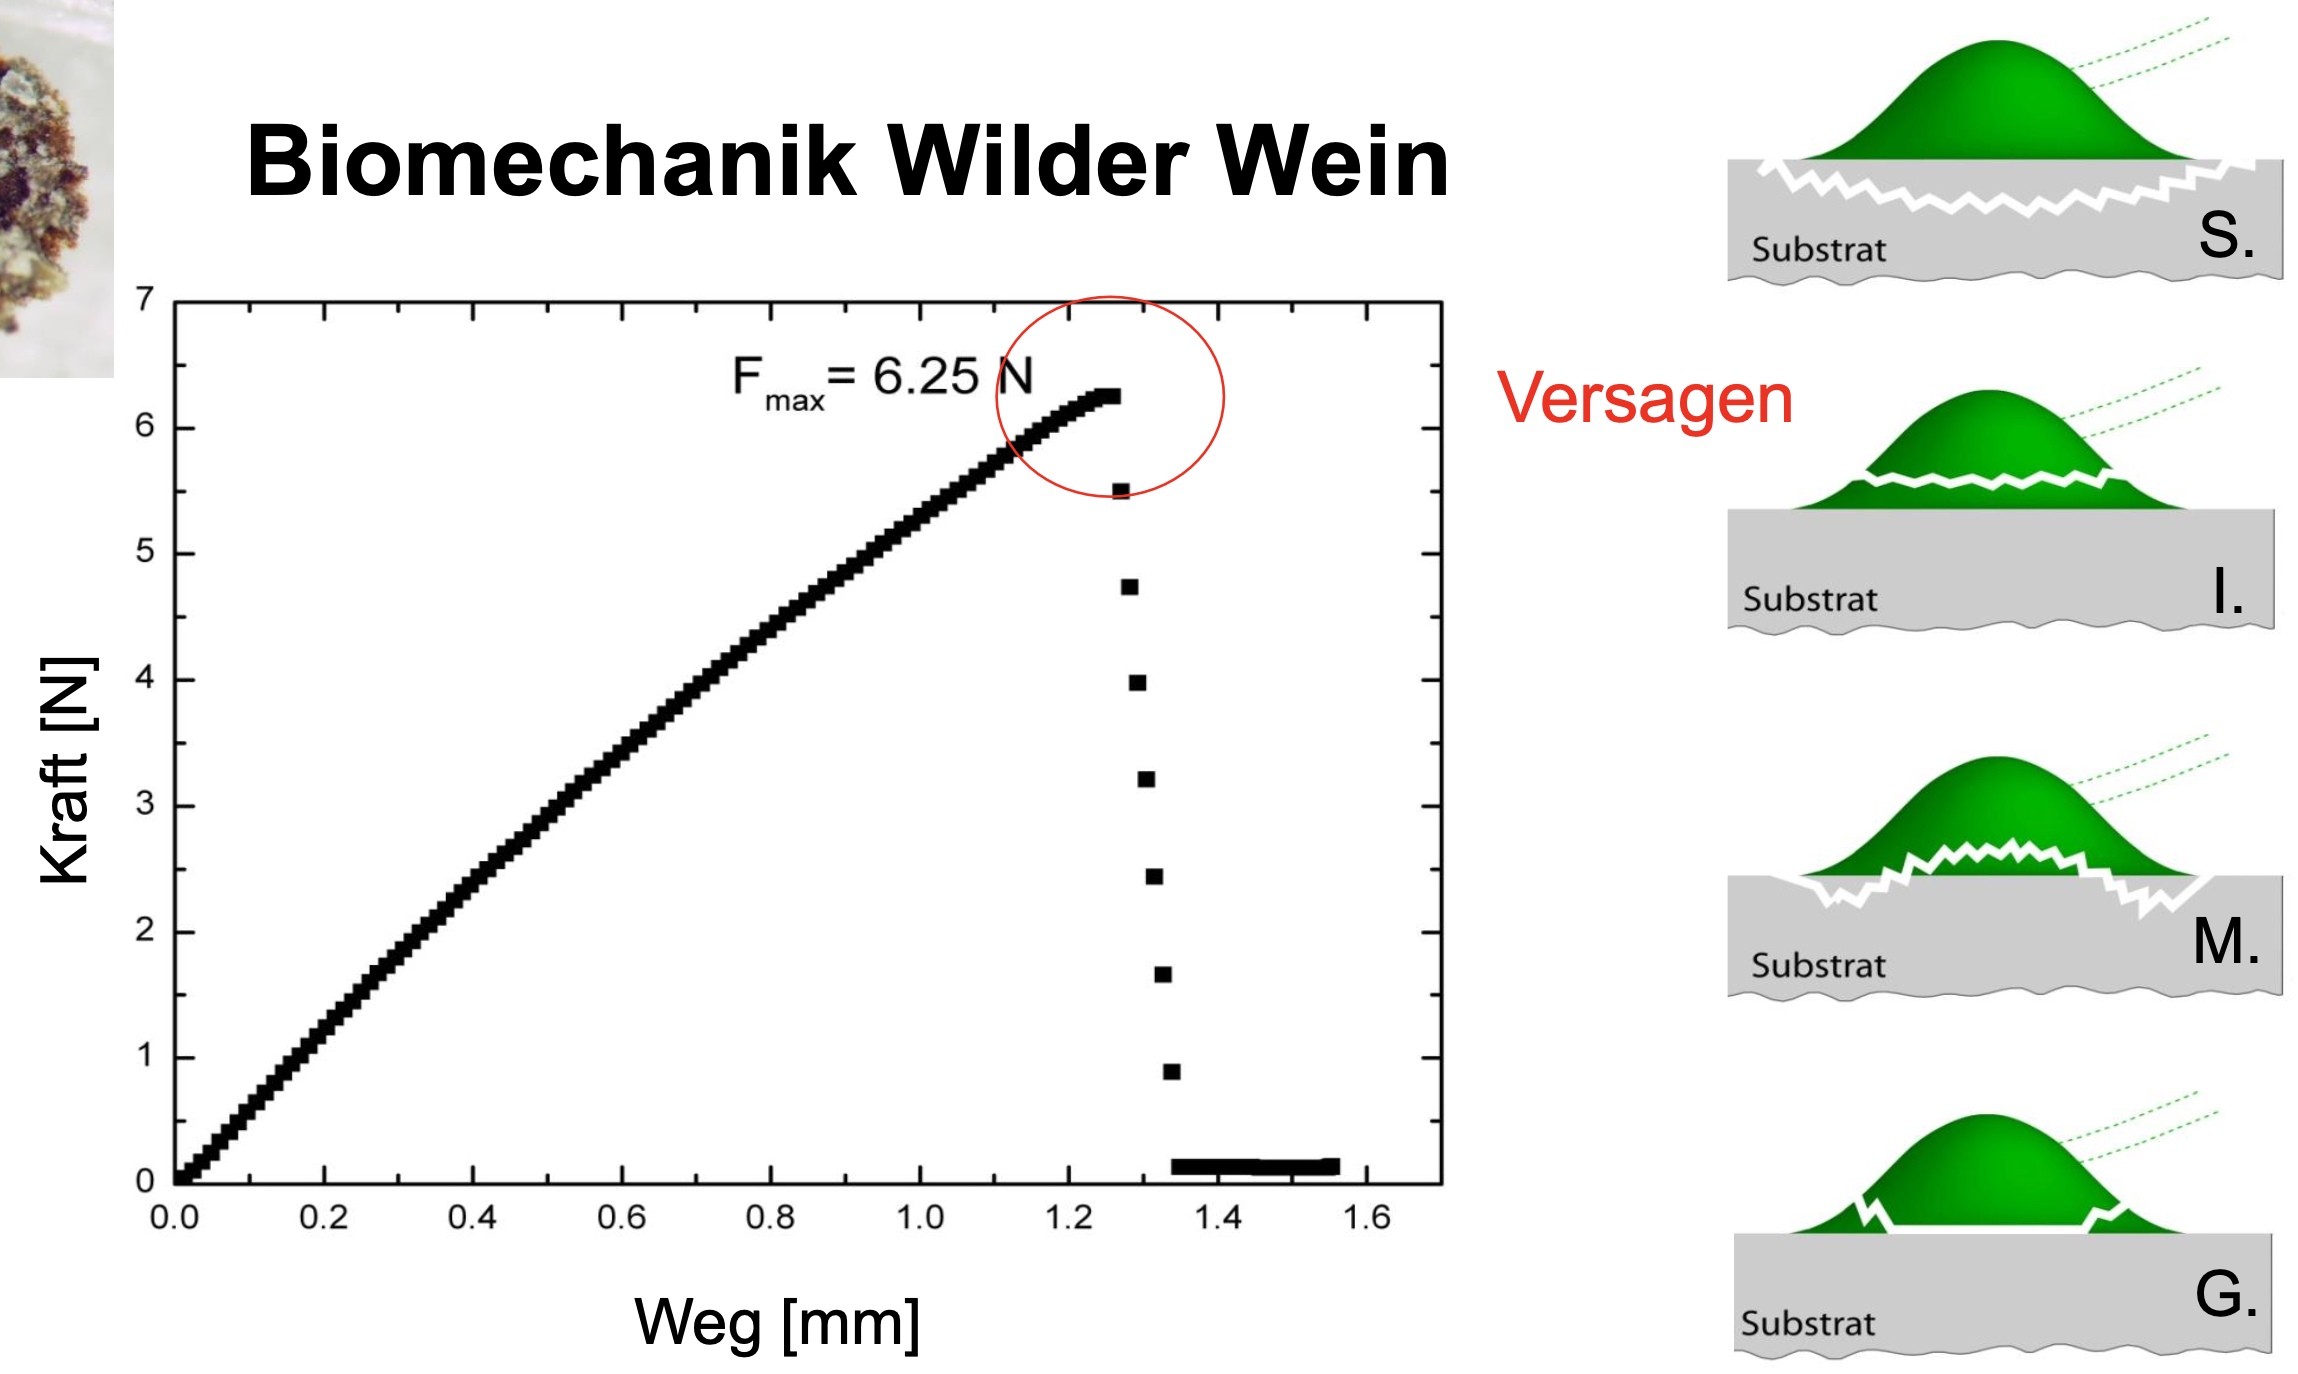
\includegraphics[width=7cm]{lec4/figures/wein_versagen.png}
\end{center}

\subsection{Technische Antihaftoberflächen nach dem Vorbild von „schlecht begehbaren“ Blattoberflächen}

\textbf{Beispiel 1:} Manche Blattoberflächen sind von Insekten schlecht begehbar. Im Versuch wird die Laufkraft von Insekten auf unterschiedlichen Oberflächen aufgenommen. Dabei zeigt sich, dass die geringe Laufkraft auf Blattoberflächen nicht dadurch ensteht, dass die Pflanzenkutikula die ``Härchen'' der Insekten verschmutzt. Stattdessen reduzieren Strukturen auf der Blattoberfläche die effektive Kontaktfläche auf der Haftkraft ausgeübt werden kann. Solche Strukturen verhindern entweder die Entstehung von Van-der-Waals Kräften (D im rechten Bild) oder das ``Einkrallen'' in die Oberfläche (E im rechten Bild).

Technische Umsetzungen: Antihaftfolien zur Schädlingsbekämpfung.

\begin{center}
    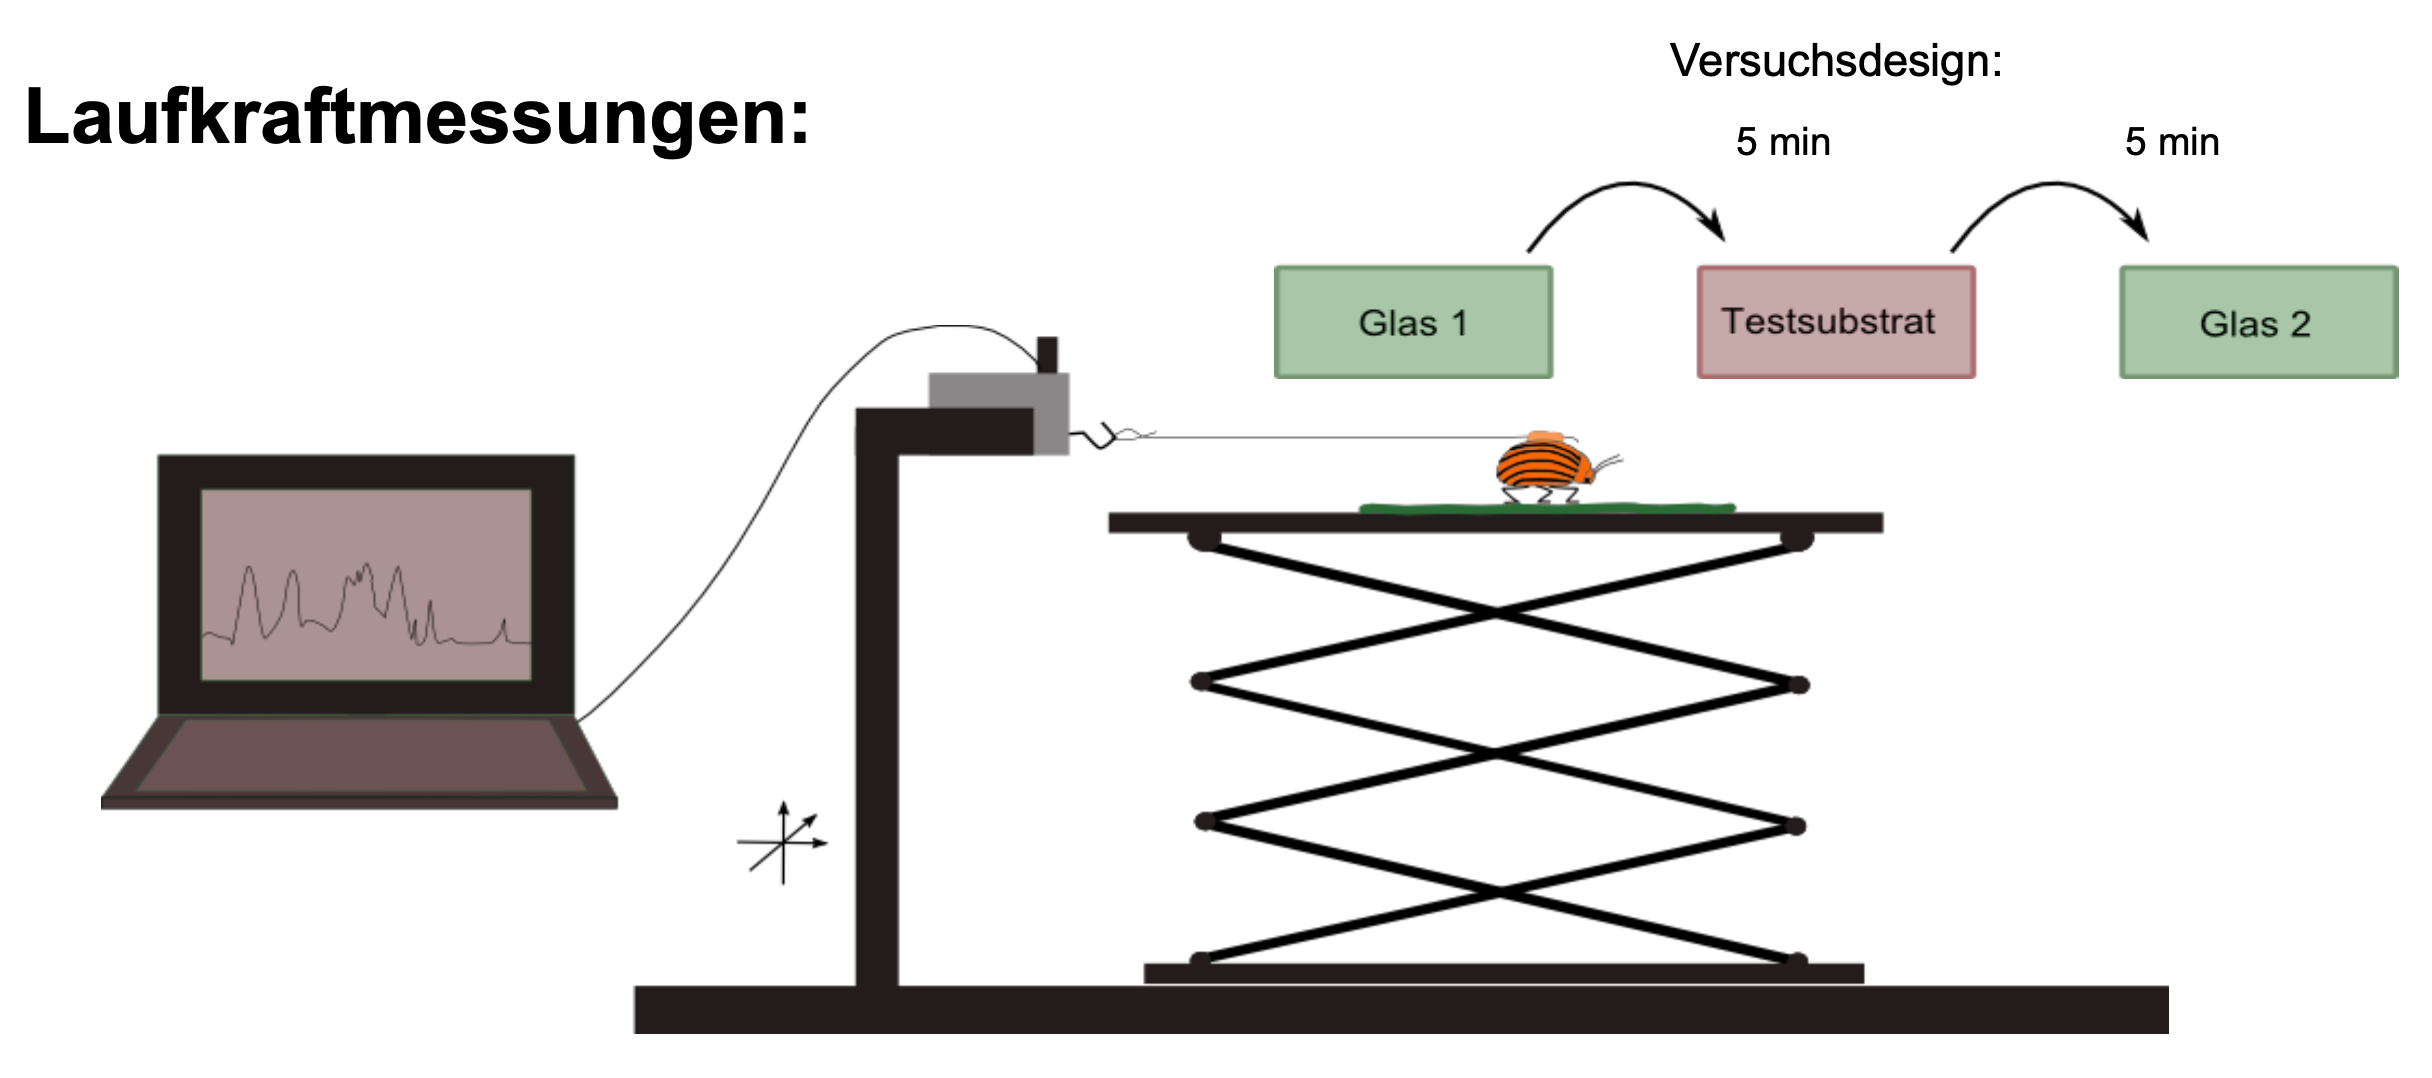
\includegraphics[width=12cm]{lec4/figures/laufkraftmessung.png}
    \hfill
    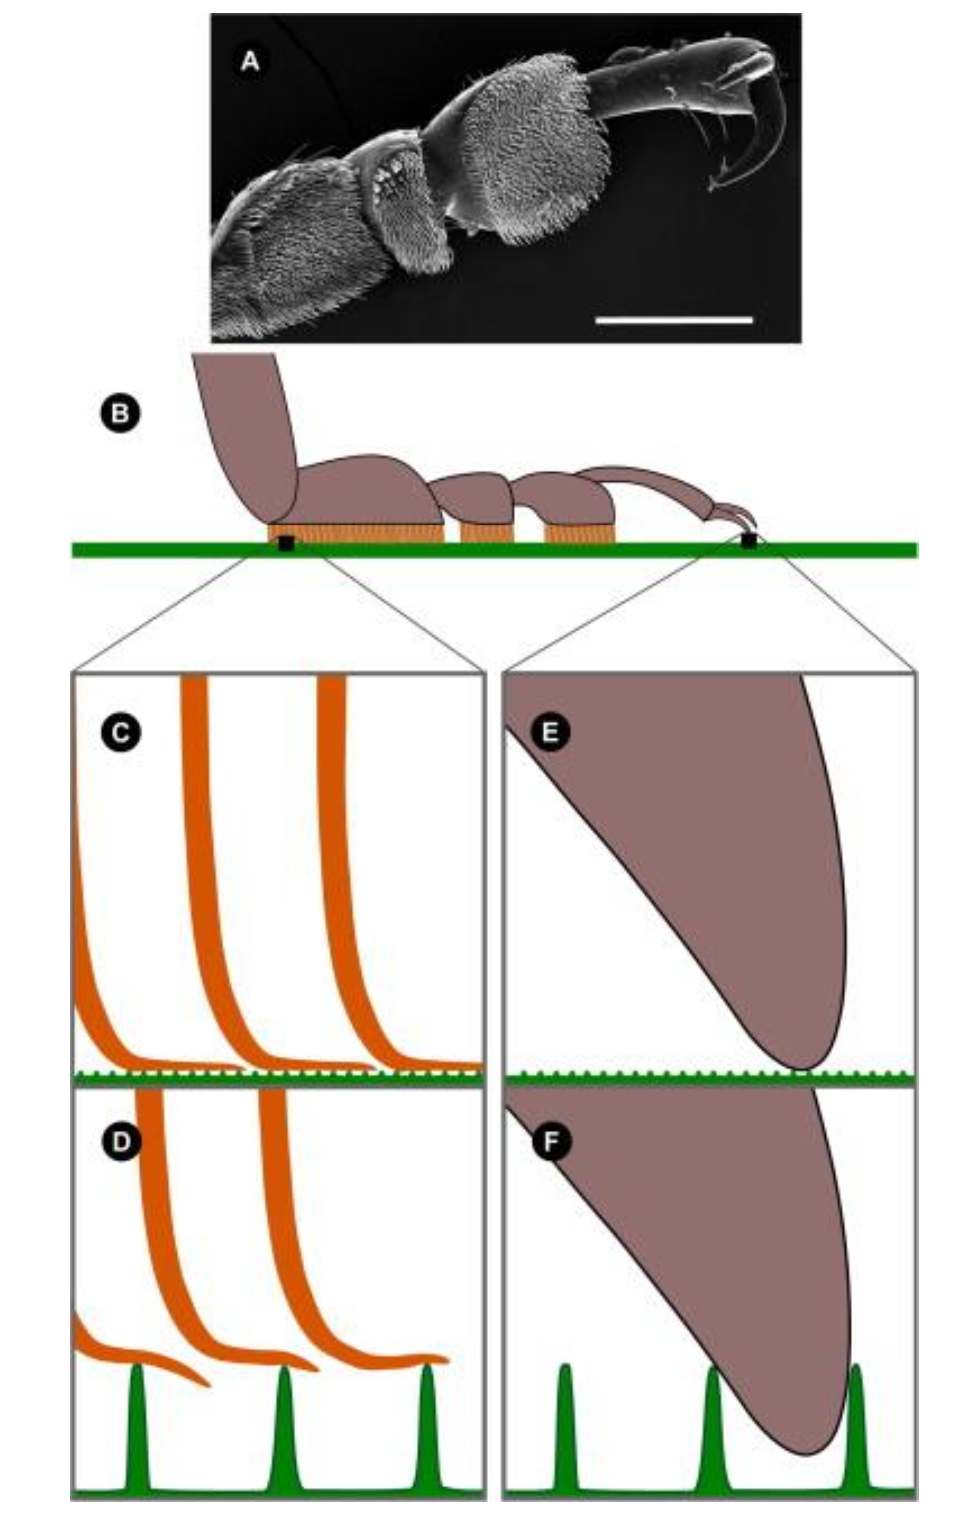
\includegraphics[width=4cm]{lec4/figures/blatt_haftung.png}
\end{center}
\textbf{Beispiel 2: Fleischfressende Pflanzen als Vorbild für Antihaft-Beschichtungen.} Ameisen rutschen an der inneren Wand ab. Die Oberfläche der Pflanze hat eine schwammartige Struktur und eine technische, ähnliche Funktions-Oberfläche (grün im Bild rechts) muss 3 Kriterien erfüllen \dangersign:
\begin{enumerate}
    \item Der Schmierfilm muss in das Substrat eindringen können
    \item Der strukturierte Festkörper muss vom Schmierstoff besser benetzt werden als von der abzuweisenden Flüssigkeit
    \item Die beiden Flüssigkeiten dürfen nicht miteinander mischbar sein $\rightarrow$ \textcolor{red}{Schmierfilmbildung}
\end{enumerate}
Ein Vorteil dieser Funktions-Oberfläche ist, dass sie \textit{auch bei Rissen abweisend} bleibt und aufgrund der Schmierflüssigkeit in der Struktur \textit{besser optisch durchlässig} ist als eine strukturierte Schicht ohne der Flüssigkeit.

\begin{center}
    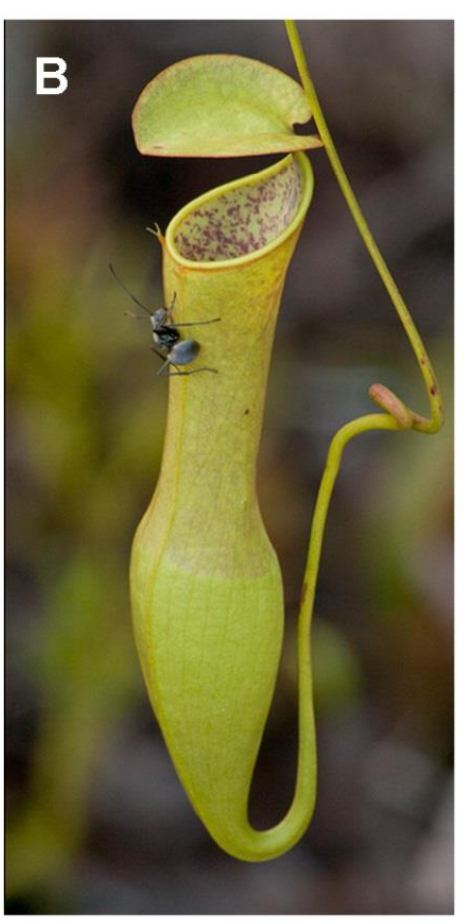
\includegraphics[width=2cm]{lec4/figures/ameise.png}
    \hfill
    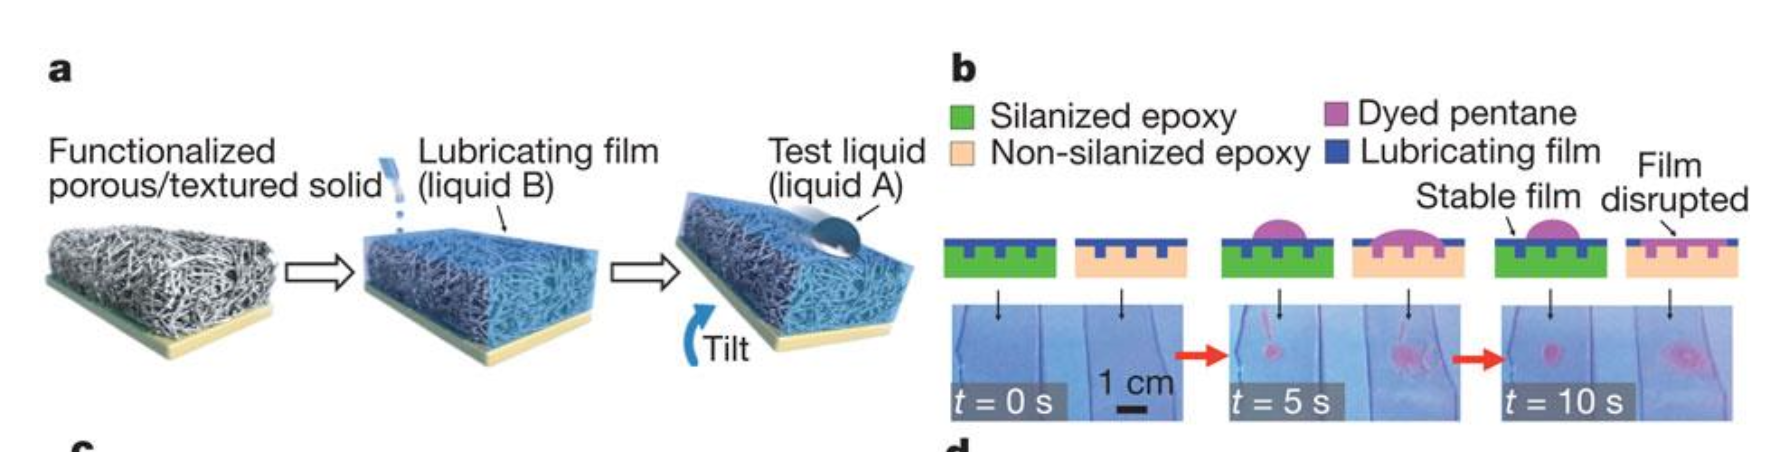
\includegraphics[width=14cm]{lec4/figures/slips.png}
\end{center}

\textit{Mögliche technische Anwendungen:} In der Medizintechnik aufgrund guter Antifouling Eigenschaften, da Bakterien nicht anhaften können (+ in der Schifffahrt). Dieser Antifouling Effekt wird allerdings nicht von der Oberfläche selbst hervorgerufen, sondern von einzer zusätzlichen aufgetragenen antibakteriellen Pflanzenschicht, welche sich in der schwammartigen Struktur einlagert. In Öl-pipelines, Optik, etc. Vorteile ggü.\ dem Lotus-Effekt sind \dangersign:

\begin{itemize}
    \item Fähigkeit auch Öle aubzuweisen
    \item Funktionieren auch unter hohem Umgebungsdruck
    \item Transparent
    \item Selbstreparatur
\end{itemize}